% Options for packages loaded elsewhere
\PassOptionsToPackage{unicode}{hyperref}
\PassOptionsToPackage{hyphens}{url}
\documentclass[
]{article}
\usepackage{xcolor}
\usepackage[margin=1in]{geometry}
\usepackage{amsmath,amssymb}
\setcounter{secnumdepth}{-\maxdimen} % remove section numbering
\usepackage{iftex}
\ifPDFTeX
  \usepackage[T1]{fontenc}
  \usepackage[utf8]{inputenc}
  \usepackage{textcomp} % provide euro and other symbols
\else % if luatex or xetex
  \usepackage{unicode-math} % this also loads fontspec
  \defaultfontfeatures{Scale=MatchLowercase}
  \defaultfontfeatures[\rmfamily]{Ligatures=TeX,Scale=1}
\fi
\usepackage{lmodern}
\ifPDFTeX\else
  % xetex/luatex font selection
\fi
% Use upquote if available, for straight quotes in verbatim environments
\IfFileExists{upquote.sty}{\usepackage{upquote}}{}
\IfFileExists{microtype.sty}{% use microtype if available
  \usepackage[]{microtype}
  \UseMicrotypeSet[protrusion]{basicmath} % disable protrusion for tt fonts
}{}
\makeatletter
\@ifundefined{KOMAClassName}{% if non-KOMA class
  \IfFileExists{parskip.sty}{%
    \usepackage{parskip}
  }{% else
    \setlength{\parindent}{0pt}
    \setlength{\parskip}{6pt plus 2pt minus 1pt}}
}{% if KOMA class
  \KOMAoptions{parskip=half}}
\makeatother
\usepackage{longtable,booktabs,array}
\usepackage{calc} % for calculating minipage widths
% Correct order of tables after \paragraph or \subparagraph
\usepackage{etoolbox}
\makeatletter
\patchcmd\longtable{\par}{\if@noskipsec\mbox{}\fi\par}{}{}
\makeatother
% Allow footnotes in longtable head/foot
\IfFileExists{footnotehyper.sty}{\usepackage{footnotehyper}}{\usepackage{footnote}}
\makesavenoteenv{longtable}
\usepackage{graphicx}
\makeatletter
\newsavebox\pandoc@box
\newcommand*\pandocbounded[1]{% scales image to fit in text height/width
  \sbox\pandoc@box{#1}%
  \Gscale@div\@tempa{\textheight}{\dimexpr\ht\pandoc@box+\dp\pandoc@box\relax}%
  \Gscale@div\@tempb{\linewidth}{\wd\pandoc@box}%
  \ifdim\@tempb\p@<\@tempa\p@\let\@tempa\@tempb\fi% select the smaller of both
  \ifdim\@tempa\p@<\p@\scalebox{\@tempa}{\usebox\pandoc@box}%
  \else\usebox{\pandoc@box}%
  \fi%
}
% Set default figure placement to htbp
\def\fps@figure{htbp}
\makeatother
% definitions for citeproc citations
\NewDocumentCommand\citeproctext{}{}
\NewDocumentCommand\citeproc{mm}{%
  \begingroup\def\citeproctext{#2}\cite{#1}\endgroup}
\makeatletter
 % allow citations to break across lines
 \let\@cite@ofmt\@firstofone
 % avoid brackets around text for \cite:
 \def\@biblabel#1{}
 \def\@cite#1#2{{#1\if@tempswa , #2\fi}}
\makeatother
\newlength{\cslhangindent}
\setlength{\cslhangindent}{1.5em}
\newlength{\csllabelwidth}
\setlength{\csllabelwidth}{3em}
\newenvironment{CSLReferences}[2] % #1 hanging-indent, #2 entry-spacing
 {\begin{list}{}{%
  \setlength{\itemindent}{0pt}
  \setlength{\leftmargin}{0pt}
  \setlength{\parsep}{0pt}
  % turn on hanging indent if param 1 is 1
  \ifodd #1
   \setlength{\leftmargin}{\cslhangindent}
   \setlength{\itemindent}{-1\cslhangindent}
  \fi
  % set entry spacing
  \setlength{\itemsep}{#2\baselineskip}}}
 {\end{list}}
\usepackage{calc}
\newcommand{\CSLBlock}[1]{\hfill\break\parbox[t]{\linewidth}{\strut\ignorespaces#1\strut}}
\newcommand{\CSLLeftMargin}[1]{\parbox[t]{\csllabelwidth}{\strut#1\strut}}
\newcommand{\CSLRightInline}[1]{\parbox[t]{\linewidth - \csllabelwidth}{\strut#1\strut}}
\newcommand{\CSLIndent}[1]{\hspace{\cslhangindent}#1}
\setlength{\emergencystretch}{3em} % prevent overfull lines
\providecommand{\tightlist}{%
  \setlength{\itemsep}{0pt}\setlength{\parskip}{0pt}}
\usepackage{bookmark}
\IfFileExists{xurl.sty}{\usepackage{xurl}}{} % add URL line breaks if available
\urlstyle{same}
\hypersetup{
  pdftitle={Manuscript\_draft},
  pdfauthor={Madeline Frazer},
  hidelinks,
  pdfcreator={LaTeX via pandoc}}

\title{Manuscript\_draft}
\author{Madeline Frazer}
\date{}

\begin{document}
\maketitle

\section{Ants, Plants, and Rats: Effects of Predator Exclusion on
Chihuahua Plant Species
Abundance}\label{ants-plants-and-rats-effects-of-predator-exclusion-on-chihuahua-plant-species-abundance}

\subsection{Introduction}\label{introduction}

Plant species abundance is a result of many abiotic and biotic factors,
including predation. Two main plant predators of Chihuahua plants
include ants and rodents.

We aimed to use existing, publicly available data by\footnote{S. K.
  Morgan Ernest, Thomas J. Valone, and James H. Brown, {``Long-Term
  Monitoring and Experimental Manipulation of a Chihuahuan Desert
  Ecosystem Near Portal, Arizona, USA,''} \emph{Ecology} 90, no. 6
  (2009): 1708--8, \url{https://doi.org/10.1890/08-1222.1}.} to
understand how each predator population (ants and rodents) influence
plant species diversity. This data set collected longitudinal data plant
abundance data, ant colony data, rodent data, and precipitation data
from 1977-2002 across 24 experimental exclusion plots.

\subsection{Materials and Methods}\label{materials-and-methods}

The data for this project is publicly available.

For treatment data, a qualitative table of the treatments each plot
received on which years can be found in the metadata for this
\href{https://www.esapubs.org/archive/ecol/E090/118/metadata.htm}{data
set}. This project includes a copy of that qualitative table in CSV form
(plot\_treatments). It also includes a quantitative version, where each
unique combination of plot and year has corresponding binary values
representing the inclusion or exclusion of kangaroo rats (large
rodents), all rodents, \emph{Pogonomyrmex rugosus} (a granivorous ant
species), or all ants. 0 = excluded (not present), 1 = included
(present). This table is what is used in the following analyses.

While the longitudinal study went from 1977-2002, we only used data from
1989--2002 because that is when plant species-level abundances were
consistently recorded.

Using the plant species data, although it was recorded for annuals and
perennials both in winter and in summer, and were measured across
quadrats within each plot, all species abundances were summed for each
plot for each year. Similarly, precipitation data was summed for a total
precipitation per year, the same for all plots of that year.

I ran a model comparison to determine what model best represented the
data. Negative binomial had an improved AICc score compared to Poisson,
so that model structure was used for future models. When comparing all
possible combinations of predictive factors (presence/absence of large
rodents, presence/absence of all rodents, presence/absence of PORU ants,
presence/absence of all ants, and precipitation), the top models
contained either presence/absence of all ants or presence/absence of
PORU ants and precipitation. Due to the more informative nature of
presence/absence of all ants compared to just PORU ants, precipitation
and the presence/absence of all ants were chosen as factors in the
Negative Binomial model.

For fixed effects, Year and Plot were added (crossed). It was determined
that keeping Year in the model made a significant difference compared to
just Precipitation, although there was some colinearity.

DHARMa residuals were imperfect, so variance was added to the model
(\textasciitilde{} Annual\_precip\_s + All\_ants * All\_rodents).
Although the presence of rodents did not predict plant abundnace, it did
help explain some of the variation in the data.

Data were checked for temporal autocorrelation, which was not found.
Spatial autocorrelation was predicted to explain the remaining variance
in the data, but was not able to be accounted for due to lack of
geographic coordinates and a precise map of the plot spacing.

It was determined that the outliers did not affect the model.

\subsection{Results}\label{results}

Here is a table of which plots had which treatment(s).

Changes in treatment assignments to the 24 experimental plots through
time. To help highlight which plots were modified, only changes in
treatment after 1985 are recorded below. Blank cells denote no changes
in treatment from the previous time period. \emph{Pogonomyrmex rugosus}
was a dominant granivorous ant species that declined at the site.
Banner-tailed kangaroo rats (\emph{Dipodomys spectabilis}) were a
dominant rodent granivore that also declined during the 1980s. (Table
modified from Brown 1998). * plot 24 was not initiated until 1979
(Samson et al.~1992)

\begin{longtable}[]{@{}
  >{\centering\arraybackslash}p{(\linewidth - 6\tabcolsep) * \real{0.0400}}
  >{\centering\arraybackslash}p{(\linewidth - 6\tabcolsep) * \real{0.3467}}
  >{\centering\arraybackslash}p{(\linewidth - 6\tabcolsep) * \real{0.3467}}
  >{\centering\arraybackslash}p{(\linewidth - 6\tabcolsep) * \real{0.2667}}@{}}
\caption{Plot Treatments}\tabularnewline
\toprule\noalign{}
\begin{minipage}[b]{\linewidth}\centering
Plot
\end{minipage} & \begin{minipage}[b]{\linewidth}\centering
X1977\_1985
\end{minipage} & \begin{minipage}[b]{\linewidth}\centering
X1985\_1987
\end{minipage} & \begin{minipage}[b]{\linewidth}\centering
X1988\_2002
\end{minipage} \\
\midrule\noalign{}
\endfirsthead
\toprule\noalign{}
\begin{minipage}[b]{\linewidth}\centering
Plot
\end{minipage} & \begin{minipage}[b]{\linewidth}\centering
X1977\_1985
\end{minipage} & \begin{minipage}[b]{\linewidth}\centering
X1985\_1987
\end{minipage} & \begin{minipage}[b]{\linewidth}\centering
X1988\_2002
\end{minipage} \\
\midrule\noalign{}
\endhead
\bottomrule\noalign{}
\endlastfoot
1 & Mixed-size seeds added in pulse & All annuals removed &
Banner-tailed kangaroo rat removed \\
2 & Small seeds added & Summer annuals removed & Unmanipulated
control \\
3 & Kangaroo ratsremoved, & & \\
Pogonomyrmex rugosus~removed & Kangaroo rats removed, & & \\
Pogonomyrmex rugosus~removed & Kangaroo rats removed, & & \\
All ants removed & & & \\
4 & All ants removed & All ants removed & All ants removed \\
5 & Banner-tailed kangaroo rats removed & Banner-tailed kangaroo rats
removed & All rodents removed \\
6 & Large seeds added & Winter annuals removed & Kangaroo rats
removed \\
7 & All rodents removed & All rodents removed & All rodents removed \\
8 & Pogonomyrmex rugosus~removed & Pogonomyrmex rugosus~removed & All
ants removed \\
9 & Mixed-size seeds added & Bi-seasonal annuals removed & Banner-tailed
kangaroo rats removed \\
10 & All rodents removed, & & \\
All ants removed & All rodents removed, & & \\
All ants removed & All rodents removed, & & \\
All ants removed & & & \\
11 & Unmanipulated control & Unmanipulated control & Unmanipulated
control \\
12 & Pogonomyrmex rugosus~removed & Pogonomyrmex rugosus~removed & All
ants removed \\
13 & Large seeds added & Winter annuals removed & Kangaroo rats
removed, \\
All ants removed & & & \\
14 & Unmanipulated control & Unmanipulated control & Unmanipulated
control \\
15 & Kangaroo rats removed & Kangaroo rats removed & Kangaroo rats
removed \\
16 & All rodents removed & All rodents removed & All rodents removed \\
17 & All ants removed & All rodents removed & All rodents removed \\
18 & Mixed-sized seeds added in pulse & All annuals removed & Kangaroo
rats removed \\
19 & Kangaroo rats removed, & & \\
Pogonomyrmex rugosus~removed & Kangaroo rats removed, & & \\
Pogonomyrmex rugosus~removed & Kangaroo rats removed, & & \\
All ants removed & & & \\
20 & Mixed-sized seeds added & Biseasonal annuals removed & Kangaroo
rats removed, \\
All ants removed & & & \\
21 & Kangaroo rats removed & Kangaroo rats removed & Kangaroo rats
removed \\
22 & Small seeds added & Summer annuals removed & Unmanipulated
control \\
23 & All rodents removed, & & \\
All ants removed & All rodents removed, & & \\
All ants removed & All rodents removed, & & \\
All ants removed & & & \\
24 & Banner-tailed kangaroo rats removed & Banner-tailed kangaroo rats
removed & All rodents removed \\
\end{longtable}

Here is a figure of how the model predicts total plant species abundance
using the presence/absence of all ants as a predictor.

\begin{verbatim}
## here() starts at C:/Users/madel/Downloads/Mini-Project
\end{verbatim}

\begin{verbatim}
## 
## Attaching package: 'dplyr'
\end{verbatim}

\begin{verbatim}
## The following objects are masked from 'package:stats':
## 
##     filter, lag
\end{verbatim}

\begin{verbatim}
## The following objects are masked from 'package:base':
## 
##     intersect, setdiff, setequal, union
\end{verbatim}

Here is a figure of how the model predicts total plant species abundance
using the total annual precipitation as a predictor.

This model still has strong variance in the residuals, as can be seen by
the DHARMa package.

\begin{verbatim}
## This is DHARMa 0.4.7. For overview type '?DHARMa'. For recent changes, type news(package = 'DHARMa')
\end{verbatim}

\begin{figure}
\centering
\pandocbounded{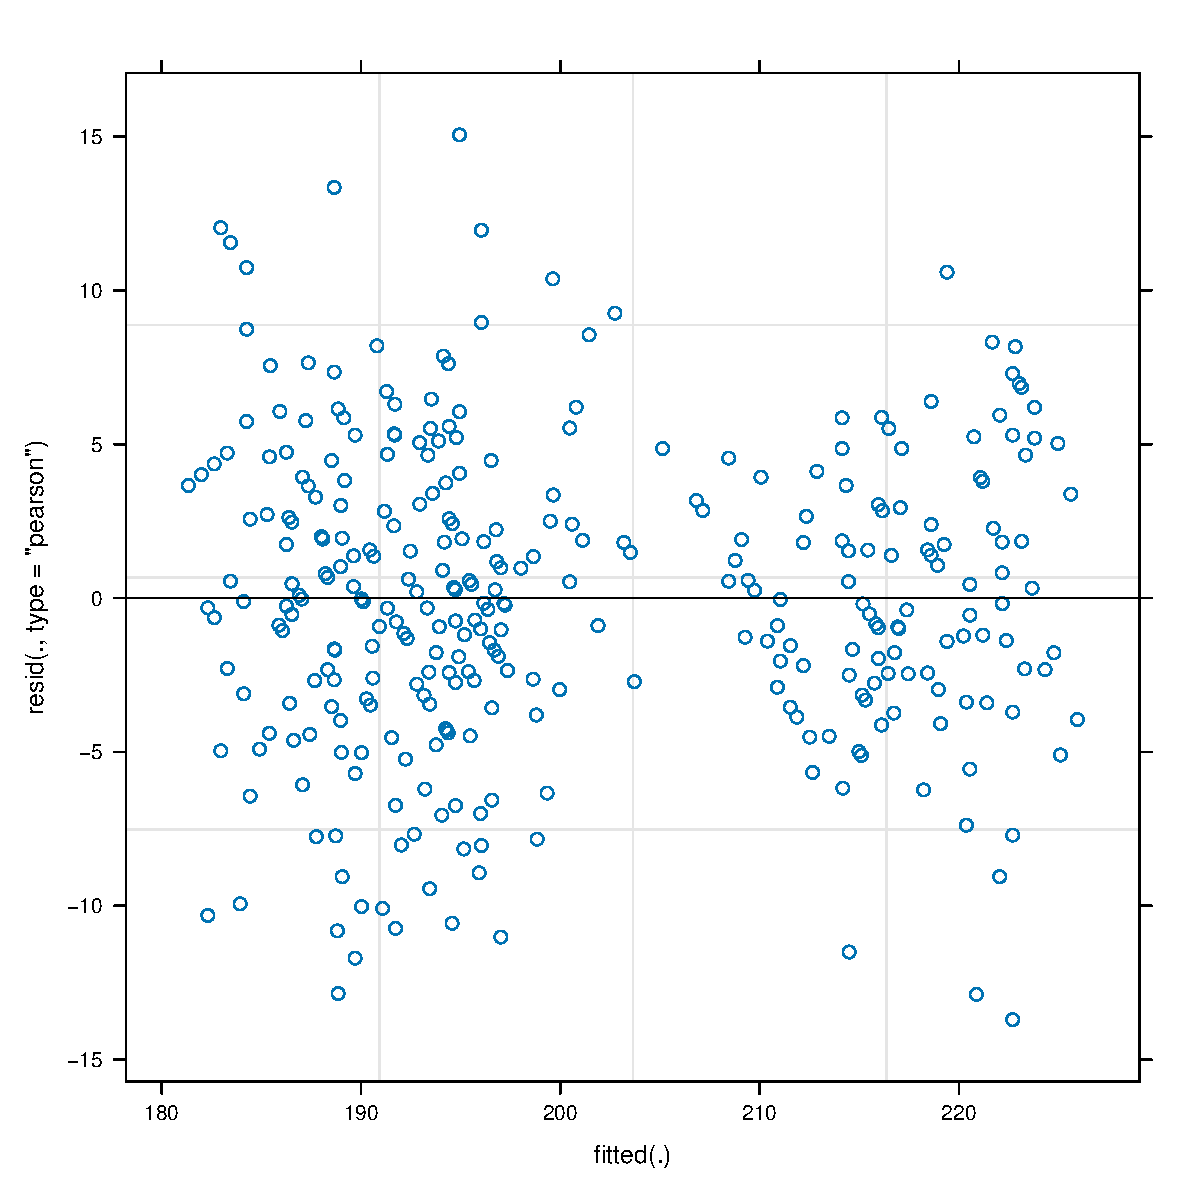
\includegraphics[keepaspectratio]{Manuscript_files/figure-latex/unnamed-chunk-4-1.pdf}}
\caption{DHARMa residuals}
\end{figure}

In conditional model, the intercept and the presence or absence of all
ants were significant predictors of total plant species abundance. The
presence of ants negatively impacted total plant species abundance by
-0.3170 (p = 0.00569). However, while the presence/absence of Rodents
helped account for variance in th model (particularly its interaction
with ants, p-value = 0.0904), it was not a significant predictor of
plant species abundance (p-value = 0.29836) Annual precipitation
(scaled) was not a significant predictor of plant species abundance
(p-value = 0.19516).

In dispersion model, annual precipitation (scaled) significantly
affected the dispersion of the model (p = 1.30e-07).

\subsection{Discussion}\label{discussion}

The presence or absence of ants on a plot was the strongest predictor of
total plant species abundance, controlling for year and plot. The
presence of ants negatively affected plant species abundance, much more
significantly than the presence of rodents on the plot, although there
is likely an interactive effect. Annual precipitation explained the
variance of total plant species abundance from the predicted model, but
was not itself a significant predictor of total plant species abundance.

\subsection{Conclusion}\label{conclusion}

Ants are a significant predator of plants and should be considered in
conservation and management plans.

\subsection*{Bibliography}\label{bibliography}
\addcontentsline{toc}{subsection}{Bibliography}

\phantomsection\label{refs}
\begin{CSLReferences}{1}{0}
\bibitem[\citeproctext]{ref-ernest2009}
Ernest, S. K. Morgan, Thomas J. Valone, and James H. Brown. {``Long-Term
Monitoring and Experimental Manipulation of a Chihuahuan Desert
Ecosystem Near Portal, Arizona, USA.''} \emph{Ecology} 90, no. 6 (2009):
1708--8. \url{https://doi.org/10.1890/08-1222.1}.

\end{CSLReferences}

\end{document}
